\documentclass[11pt]{article}

\usepackage{graphicx}
\usepackage[utf8]{inputenc}
\usepackage{hyperref}
\usepackage{mathtools}
\usepackage{float}
\usepackage[margin=0.5in]{geometry}
\usepackage{xcolor}
\hypersetup{
  colorlinks=true,
  linkcolor=blue!50!red,
  urlcolor=green!70!black
}

\begin{document}
\setlength{\textwidth}{20cm}
\setlength{\textheight}{22cm}
\title{\Huge\textbf{Neural Networks}\linebreak \small{Predicting student performance} \linebreak\linebreak
\Large\textbf{Intermediate Report}\linebreak\linebreak
\linebreak\linebreak

\includegraphics[scale=0.1]{feup-logo.png}\linebreak\linebreak
\linebreak\linebreak
\Large{Mestrado Integrado em Engenharia Informática e Computação} \linebreak\linebreak
\Large{Inteligência Artificial}\linebreak\linebreak
\Large{Group E5\_1}
}

\author{
Gonçalo Lopes\\ up201303198\\
\and
Ivo Fernandes\\ up201303199\\
}
\date{\today}
\maketitle
\newpage
\tableofcontents
\newpage

\section{Objective}

The purpose of this project is to train an Artificial Neural Network, using the Back-Propagation algorithm, in order to predict student performance based on attributes for each student, taking into account aspects of the student's private and work life and also attributes like their gender and age.

\section{Description}
\subsection{Specification}

\subsubsection{Project phases}
\label{sec:phases}
To complete this project the group will have to:
\begin{enumerate}
\item Understand the structure of a neural network
\item Understand the mechanism of the back-propagation algorithm
\item Choose a back-propagation framework and learn it
\item Learn how to train neural networks
\item Build different networks and train them
\item Compare the networks, try different training methods, handle the data-set
\item Construct a final network and evaluate its accuracy
\end{enumerate}

\subsubsection{Network Structure}
\label{sec:network}
A neural network is comprised of 3 types of layers, each layer containing nodes that represent neurons.
\begin{itemize}
\item Input Layer
\item Hidden Layers
\item Output Layer
\end{itemize}

Each layer can have a different number of nodes and all of a layer's nodes are connected to all of the next layer's nodes. There is only one input layer and one output layer. There can be any number of hidden layers, each with any number of nodes. To solve most problems, only one hidden layer is required. Usually, the output layer consists of a single node.
A neuron consists of 5 main parts:
\begin{enumerate}
\item The \textbf{input}, through which the neuron receives information
\item The \textbf{connection weights}, that determine how much influence each input value has
\item The \textbf{combination function}, which is usually a sum of the input values times their respective weights
\item The \textbf{activation function}, which calculates the state of the neuron. The function used is usually the sigmoid function $\frac{1}{1+e^{-\alpha}}$ This function is used because it introduces non-linearity in the network, as opposed to using a step function. This function is also continuous and differentiable. Take $\beta = \frac{1}{1+e^{-\alpha}}$, $\frac{\partial\beta}{\partial\alpha}$ = $\beta (1-\beta)$
\item The \textbf{output}, which is the result of the transfer function. If we didn't introduce non-linearity by using the sigmoid function, output $s_i \in \{0, 1\}$. Since we introduced non-linearity, output $s_i \in [0, 1]$.
\end{enumerate}
\begin{figure}[H]
\label{fig:example}
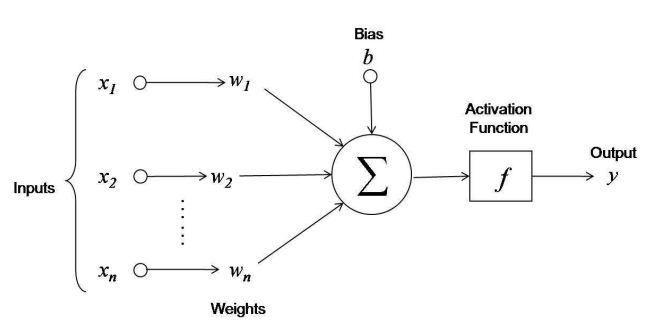
\includegraphics[scale=0.5]{neuron.jpg}
\centering
\caption{Example of a neuron, taken from \url{https://blogs.cornell.edu/info2040/2015/09/08/neural-networks-and-machine-learning/}}
\end{figure}
\hfill \break
\hfill \break

\subsubsection{Back-propagation Algorithm}
\label{sec:back}
Let $\overrightarrow{z}$ = $f(\overrightarrow{x}, \overrightarrow{w}), \overrightarrow{z}$representing the output of the neural network for the set of inputs $\overrightarrow{x}$ and set of weights $\overrightarrow{w}$
Let $\overrightarrow{d}$ = $g(\overrightarrow{x}), \overrightarrow{d}$ representing the desired output of the neural network for the set of inputs $\overrightarrow{x}$
To calculate how well the network is doing we must calculate a function that includes the difference between $\overrightarrow{d}$ and $\overrightarrow{z}$.
Let P($\overrightarrow{d}, \overrightarrow{z}$) = $\frac{1}{2} || \overrightarrow{d} -  \overrightarrow{z} ||$, we will call this the Performance function.
\hfill \break
\hfill \break
We want to minimize the Performance function, minimizing it means minimizing the difference between the desired output and the real output, which means this is the direction to go, to make the network learn.

For explaining the back-propagation algorithm we will always refer to a simple network with 1 input node and 1 hidden node.
For a network with 2 nodes, 2 weights, w1 and w2, $\Delta w = r(\frac{\partial P}{\partial w_1} , \frac{\partial P}{\partial w_2})$, r is the \textbf{learning rate}. As the name suggests, the learning rate will help the network learn faster, however, this rate cannot be too high. If the learning rate is too high, while trying to fit to the curve of the desired weights, the algorithm will get into a feedback loop, never converging to the minimum and learning nothing.
\begin{figure}[H]
\label{fig:example}
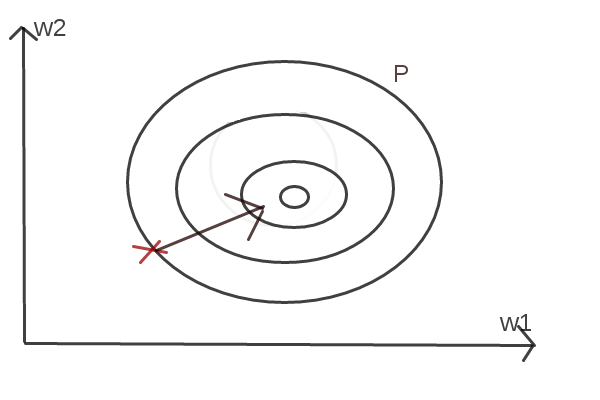
\includegraphics[scale=0.3]{performance.png}
\centering
\caption{For 2 weights, w1 and w2, we are trying to move in the direction that minimizes the P function}
\end{figure}
Since we picked the sigmoid function for our activation function, calculating $\Delta \overrightarrow{w}$ becomes simple.
Let:
\begin{itemize}
\item x be the input of node 1
\item y be the output of node 1, input of node 2
\item z be the output of node 2, the output of the network
\end{itemize}

$\frac{\partial P}{\partial w_2} = (d-z)z(1-z)y$

$\frac{\partial P}{\partial w_1} = (d-z)z(1-z)yw_2x(1-y)$

But we already calculated $(d-z)z(1-z)y$, which is $\frac{\partial P}{\partial w_2}$

This means that a given node's weight depends on the node's input, output, the weight of the next node and the partial derivative of the next node.
This gives the back-propagation algorithm its name. We propagate the error, $\frac{\partial P}{\partial w_2}$, backwards, in order to calculate $\Delta \overrightarrow{w}$, the vector containing the error for each weight.

By using multiple iterations, the algorithm adjusts the weights of the network, minimizing the performance function.

\begin{figure}[H]
\label{fig:example}
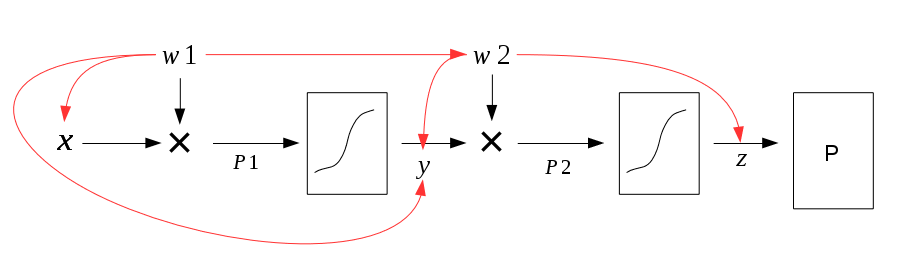
\includegraphics[scale=0.4]{example.png}
\centering
\caption{Example network with 1 input node and 1 hidden node, red arrows represent dependence.}
\end{figure}

The calculation of $\Delta \overrightarrow{w}$ may also be influenced by \textbf{momentum}. To incorporate momentum into the calculation, the new formula is:

$\Delta \overrightarrow{w}(t) = r(\frac{\partial P}{\partial w_1} , \frac{\partial P}{\partial w_2}) + m \Delta \overrightarrow{w}(t-1)$, t is the iteration number, m the momentum constant. The momentum is usually set to a high value between 0 and 1.

When we calculate $\Delta w$ we are going along the gradient of the activation function, in the direction specified by the output error. If by going along this direction, we skip the ideal point for the weights, we must go back. Momentum helps with this situation, if the algorithm was moving in a direction and it suddenly changes directions, the first step will be small, since it takes into account the direction of the last step, which was opposite to the direction of the new step.
\hfill \break
\hfill \break
A factor that may lead to unsuccessfully training the network is the number of iterations. If the number of iterations is too high overfitting may start to happen. Over fitting is when the algorithm tries so hard to fit to the sample (training set) that values nearby the ones used may become distorted, and when faced with a similar situation the network will output a very different value.
\hfill \break
\hfill \break
The back-propagation algorithm must also shuffle the dataset instances before starting each iteration, otherwise it will be unable to successfully train. The chosen framework does this.
\subsubsection{Training a series of Networks for the same dataset}
\label{sec:training}
The data-set to be used on the project has \href{http://archive.ics.uci.edu/ml/datasets/Student+Performance}{\underline{33 attributes and 649 instances}}.
The 33rd attribute of the data-set is the final grade, this will be our single output node. This means that, initially, there will be 32 input nodes.
One of the main purposes of the project, is treating the dataset, reducing non-important attributes. This will make the network training more efficient, since there will be less nodes to weight.

The framework we will be using restricts the inputs and outputs to be in the range [0, 1], so to train and test our network we need to first parse the data and transform all the inputs into the corresponding value in the range [0, 1].
\hfill \break
\hfill \break
To train and test the network we will have to divide the dataset into two separate groups. The \textbf{Training Set} and the \textbf{Test Set}, these groups will be used to train different networks, however, they will be the same for all the networks. We could use a \textbf{Validation Set}, but since we only have 649 instances, having 3 disjoint sets would mean small sets, thus, we chose not to use the Validation Set, which may or may not be used in the training of a neural network.

We will keep the Training Set size at 2/3 of the number of instances and the Test Set at 1/3, as it is usual to follow this approach.
\hfill \break
\hfill \break
As described in the \hyperref[sec:network]{Network} section, the network may have any number of hidden layers, each with any number of nodes. We must fiddle with these values while creating different networks, in order to create better networks with faster training times and better accuracy.
\hfill \break
\hfill \break
The network's learn rate and momentum may also be adjusted. We already discussed where these attributes affect the algorithm in the \hyperref[sec:back]{previous} section.
\hfill \break
\hfill \break
We can also adjust the error threshold to be achieved, which means that when the back-propagation calculated error is below the threshold, the training of the network stops.
\subsection{Expected Results and Tests}
From training different networks, and fiddling with the attributes referenced in the \hyperref[sec:training]{training} section, we expect to see different training times and network accuracies.

We are unable to set an accuracy goal for our final network, but we hope to see a noticeable increase when comparing our final network to our first.

\newpage
\section{Development}
The project is being developed on Debian "Jessie".

We are using \href{https://github.com/harthur/brain}{\textbf{BrainJS}}, as our neural network framework.

Since we are using a Javascript framework, we decided to create a web interface, using HTML, CSS and Javascript, that allows us to change training options, create, save and load data sets  and train networks, automatically calculating:

\begin{itemize}
\item Number of iterations
\item Error threshold achieved in training
\item Training time
\item Pass course accuracy
\item Final grade accuracy
\end{itemize}

\textbf{Pass course accuracy} is defined by the network's ability to predict if a student will pass or fail the course. While testing, the network compares to expected grade to the predicted grade, after rounding the predicted grade. If both grades are greater or equal to 10, or both are lower than 10, it's a \textbf{yes} for the \textbf{Pass course accuracy}, otherwhise, it's a \textbf{no}.

\textbf{Final grade accuracy} is defined by the network's ability to predict a student's final grade. While testing, the network compares to expected grade to the predicted grade, after rounding the predicted grade. If both grades are equal, then it's a \textbf{yes} for the \textbf{Final grade accuracy}, otherwhise, it's a \textbf{no}.
\hfill \break
\hfill \break
The implementation allows us to feed in a data-set, which creates the Training and Test Set according to the inputed sizes.

For this project we will be analysing two different data sets, the portuguese and math sets. Since the students in each data set are different, the sets must be handled separately. We will only create one training and test set for each data set, in order to use the same sets for all the experiments. The Training Sets are 70\% of the data set and the Test Sets the remaining 30\%.

On the created web interface, we are also allowed to manipulate the number of hidden layers and hidden nodes, and input and output nodes. This way we can easily remove some nodes from the neural network and perform experiments.

\section{Experiments}
In this section, we will perform all the experiments and discuss the results.

The objective of the experiments is to identify the optimal neural net structure and identify which inputs really affect the output. This is done so that the neural network trains in the least amount of time and the training results are the best possible with the current data set available.

When specifying the number of hidden layers and hidden nodes used, the following representation is used:
\textit{\{nodes\_First\_layer, nodes\_Second\_layer, ...., nodes\_N\_layer\}}

The removed column on the tables specifies the input nodes that were removed for that execution.

Since the used framework is based on Javascript, training times will be higher than if a Java or C++ framework was used. However, iteration growth will be the same. We will only present the number of iterations for each train+test, not specifying the time. The time may also vary from what other work the browser is doing, which means it would not be a very meaningful metric.

The training and test sets are obtained only once for each data-set. These sets are obtained after shuffling the data-set, in order to achieve plausible results. If the data-set was not shuffled, the train set might contain very similar instances, and all of them very different from the instances on the test set, which would lead to bad accuracy.

Since the data-set is only shuffled once to create the training and test set. Maybe the resulting shuffle is a bad one, this means that all following experiments will have either all higher or all lower results on experiments, however, the difference between experiments will still be noticeable. Nonetheless, this wouldn't happen if the original data-set was large and representative enough. Which does not happen because the Math dataset has less than 400 instances, and the Portuguese one, less than 700, which is clearly not enough, given the number of features presented on the sets.

The training set is also shuffled between each training iteration. This means different training runs may yield different test reults, even though the sets are the same.

\subsection{The quitters}
A quitter is a student who either failed the course due to too many absences, or decided to drop out. This means the quitter will have a G3 of 0.

We will use the Math dataset for this experiment, the same result is expected from the Portuguese dataset.

Using the \textbf{default data-set:}

\begin{tabular}{| c | c | c | c | c | c | c | c |}
\hline \textbf{min\_thresh} & \textbf{hidden} & \textbf{learn\_rate} & \textbf{momentum} & \textbf{removed} & \textbf{iterations} & \textbf{PassAcc} & \textbf{GradeAcc}\\
\hline 0.005 & \{1\} & 0.3 & 0.8 & \_ & 260 & 90\% & 64\%\\
\hline 0.0005 & \{1\} & 0.3 & 0.8 & \_ & 1693 & 80\% & 41\%\\
\hline 0.0005 & \{1\} & 0.2 & 0.9 & \_ & 2380 & 81\% & 49\%\\
\hline 0.0005 & \{5\} & 0.2 & 0.9 & \_ & 2519 & 82\% & 46\%\\
\hline 0.0005 & \{10,5\} & 0.2 & 0.9 & \_ & 2457 & 81\% & 40\%\\
\hline
\end{tabular}

\hfill \break
\hfill \break
Using the \textbf{no-quitters data-set:}

\begin{tabular}{| c | c | c | c | c | c | c | c |}
\hline \textbf{min\_thresh} & \textbf{hidden} & \textbf{learn\_rate} & \textbf{momentum} & \textbf{removed} & \textbf{iterations} & \textbf{PassAcc} & \textbf{GradeAcc}\\
\hline 0.005 & \{1\} & 0.3 & 0.8 & \_ & 19 & 91\% & 70\%\\
\hline 0.0005 & \{1\} & 0.3 & 0.8 & \_ & 1666 & 89\% & 64\%\\
\hline 0.0005 & \{1\} & 0.2 & 0.9 & \_ & 1987 & 86\% & 59\%\\
\hline 0.0005 & \{5\} & 0.2 & 0.9 & \_ & 2218 & 92\% & 63\%\\
\hline 0.0005 & \{10,5\} & 0.2 & 0.9 & \_ & 2057 & 93\% & 62\%\\
\hline
\end{tabular}

\hfill \break
\hfill \break

For the default set, with the default min threshold, the pass accuracy is the same as for the no-quitters set. After lowering the min threshold 10 times, the pass accuracy stays the same for the no-quitters set but drops almost 10\% on all the following experiments for the default set. As for the grade accuracy, it drops an average of 7\% for the no-quitters set and an average of 20\% for the default set. This is due to overfitting, and this is why the experiments included lowering the learning rate and momentum and changing hidden layers. However, the obtained results were not much different.
\hfill \break
\hfill \break
\newpage
\textit{Why do both sets suffer from overfitting?}

This happens because, as already referenced, the datasets are small and not very representative.

\textit{Why does grade accuracy drop more on the default set than pass accuracy, when compared to the value changes for the no-quitters set?}

Because when a student has a 0, and the network calculates for example a 5 for that student, even though the grade error is large, the pass result is still the same.

\begin{figure}[H]
\label{fig:Pass vs Grade}
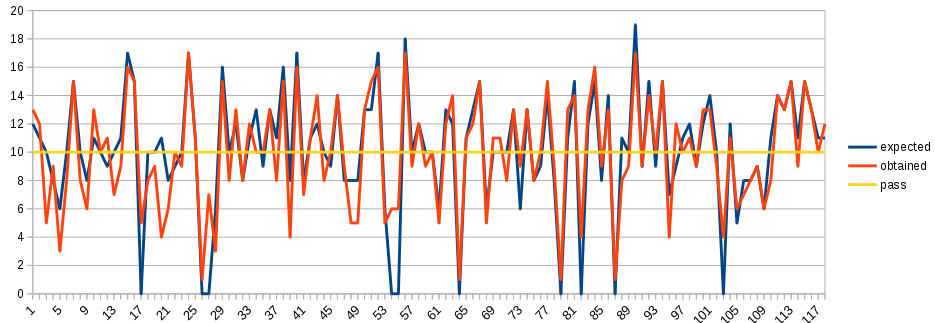
\includegraphics[scale=0.6]{passgrade.png}
\centering
\caption{Pass vs Grade accuracy (default)}
\end{figure}

The pass accuracy only fails when the expected and obtained values are on different sides of the pass line. This did not happen for any of the quitters.

\begin{figure}[H]
\label{fig:Pass vs Grade}
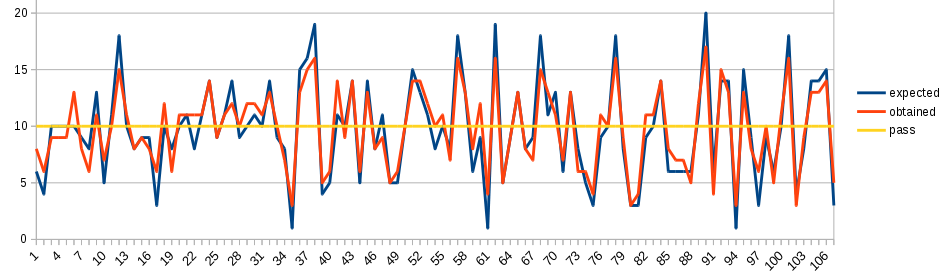
\includegraphics[scale=0.6]{passgradenoquit.png}
\centering
\caption{Pass vs Grade accuracy (no-quitters)}
\end{figure}

\newpage
\textit{Why does the default set have worse results than the no-quitters set?}

Because there is more overfitting on the default set, due to quitters. A quitter might have the same input values as someone who passed the course, but because of quitting, the result is 0. This leads to the network giving lower grades to students that did not quit.

When comparing both graphs, we can clearly see the default network overfitting students and giving them a lower grade, while also giving quitters a higher grade than 0.

\hfill \break
\hfill \break

We can also observe on the 2 graphs that, due to data-set shuffling, the default test set had no students with G3 of 20, while the no-quitters set had a student with a G3 of 20. Having a 20 on the test set will reduce grady accuracy because it is hard to predict a 20, since it is the highest value possible. We can see on the graphs that high expected grades have lower obtained values and low expected grades have higher obtained values. The obtained values tend towards the mean.

\hfill \break
\hfill \break
\textbf{Conclusion:}

The following experiments will all be done on the no-quitters data-set.

\subsection{G1 and G2}
We expect G1 and G2 to be have a very strong influence on the result of G3, so we will test that.
\hfill \break
\hfill \break
\begin{tabular}{| c | c | c | c | c | c | c | c |}
\hline \textbf{min\_thresh} & \textbf{hidden} & \textbf{learn\_rate} & \textbf{momentum} & \textbf{removed} & \textbf{iterations} & \textbf{PassAcc} & \textbf{GradeAcc}\\
\hline 0.005 & \{1\} & 0.3 & 0.8 & \_ & 19 & 91\% & 70\%\\
\hline 0.005 & \{1\} & 0.3 & 0.8 & \_G1\_G2\_ & 467 & 59\% & 24\%\\
\hline 0.005 & \{1\} & 0.3 & 0.8 & \_G2\_ & 276 & 90\% & 45\%\\
\hline 0.005 & \{1\} & 0.3 & 0.8 & \_G1\_ & 21 & 89\% & 70\%\\
\hline
\end{tabular}

When removing both G1 and G2, pass accuracy drops 1/3 and the grade accuracy drops 2/3. As expected, the grade accuracy always drops more than the pass accuracy.
\hfill \break
\hfill \break
When removing either G1 or G2, the pass accuracy stays more or less the same. This happens because knowing a student's grades on G1 or G2 has a high impact on predicting if the student will pass or not.
\hfill \break
\hfill \break
When removing G1, the grade accuracy is almost half of when removing G2. This is because the G2 grade is a lot closer to the G3 grade than the G1. The value of G2 is depends on the value of G1, so, having G2 and not having G1 means that G1 still has some effect on the result.

We chose to perform our following experiments without G1 or G2 on our input nodes. We found it to be more interesting to detect how high can the accuracy of the network go without these input nodes, as predicting a student's grades while having the grades as input doesn't sound like predicting at all.

The following experiments will be done separately for the Math students data set and for the Portuguese students data set, as the data is from different students, we are unable to join the data and have a network with 2 outputs, which would be one for Math G3 and another for Portuguese G3.


\subsection{Math}
\begin{figure}[H]
\label{fig:Grade Distribution for Mathematics}
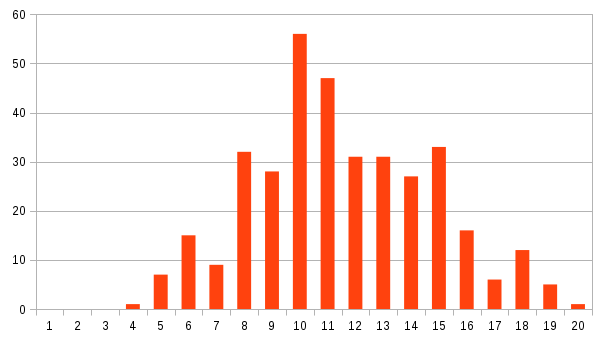
\includegraphics[scale=0.6]{mat-chart.png}
\centering
\caption{Grade Distribution for Mathematics}
\end{figure}

\subsubsection{Training threshold}
For the training threshold, we will test an array of different values. However, we suspect the training threshold of 0.025 to the best threshold. A grade is accurately defined if $|expected - obtained| < 0.5$. Seeing as all our values are mapped to [0, 1] interval, and $0.5 / 20 = 0.025$, the network is trained enough. If the network is trained any further it will start overfitting.

\begin{tabular}{| c | c | c | c | c | c | c | c |}
\hline \textbf{min\_thresh} & \textbf{hidden} & \textbf{learn\_rate} & \textbf{momentum} & \textbf{removed} & \textbf{iterations} & \textbf{PassAcc} & \textbf{GradeAcc}\\
\hline 0.0005 & \{1\} & 0.3 & 0.8 & \_G1\_G2\_ & 1178 & 55\% & 18\%\\
\hline 0.025 & \{1\} & 0.3 & 0.8 & \_G1\_G2\_ & 110 & 70\% & 29\%\\
\hline 0.005 & \{1\} & 0.3 & 0.8 & \_G1\_G2\_ & 490 & 64\% & 21\%\\
\hline 0.0005 & \{1\} & 0.3 & 0.8 & \_G1\_G2\_ & 1178 & 55\% & 18\%\\
\hline
\end{tabular}

As expected, the minimum threshold of 0.025 was the best.

\subsubsection{Removing Inputs}
In this section we will try different combinations of
\begin{itemize}
\item Input nodes
\item Hidden layer setups
\item Training values
\end{itemize}

Before testing, we expect inputs like \textit{sex, age, address, health} to not help the network predicting the values. We will begin by removing these inputs.


\begin{tabular}{| c | c | c | c | p{3cm} | c | c | c |}
\hline \textbf{min\_thresh} & \textbf{hidden} & \textbf{learn\_rate} & \textbf{momentum} & \textbf{removed} & \textbf{iterations} & \textbf{PassAcc} & \textbf{GradeAcc}\\
\hline 0.025 & \{1\} & 0.3 & 0.8 & \_G1\_G2\_ & 110 & 70\% & 29\%\\
\hline 0.025 & \{1\} & 0.3 & 0.8 & \_sex\_age \_address\_health \_G1\_G2\_ & 136 & 70\% & 32\%\\
\hline
\end{tabular}

The health input, according to the dataset, was the student's health status, at the moment of answering the questions, this means that the health value may not have had an impact on the grades, throughout the year, because the student's health status may have changed after the end of the school year.

As expected, none of these inputs help the network.
\hfill \break
\hfill \break

After a quick look at the data sets, we can see that there are only 2 schools, \textit{Gabriel Pereira} and \textit{Mousinho da Silveira}. Seeing as only 2 schools are in the data set, if both schools' students have different average grades, the network output will be worse, if the school input node is removed.

\begin{tabular}{| c | c | c | c | p{3cm} | c | c | c |}
\hline \textbf{min\_thresh} & \textbf{hidden} & \textbf{learn\_rate} & \textbf{momentum} & \textbf{removed} & \textbf{iterations} & \textbf{PassAcc} & \textbf{GradeAcc}\\
\hline 0.025 & \{1\} & 0.3 & 0.8 & \_sex\_age \_address\_health \_G1\_G2\_ & 136 & 70\% & 32\%\\
\hline 0.025 & \{1\} & 0.3 & 0.8 & \_school\_sex \_age\_address \_health\_G1\_G2\_ & 176 & 70\% & 34\%\\
\hline
\end{tabular}

From the result we can say that the average and standard deviation of the grades from different schools will be the same.

Now we will calculate the average and standard deviation for each school.

\begin{tabular}{| c | c | c |}
\hline \textbf{School} & \textbf{Average Grades} & \textbf{Standard Deviation}\\
\hline MS & 10.79 & 3.06\\
\hline GP & 11.62 & 3.24\\
\hline
\end{tabular}

As hinted by the result of removing the school input node, the average and standard deviation of the grades are fairly similar.

\newpage
We will keep trying out node input combinations until getting the best network.

\begin{tabular}{| c | c | c | c | p{3cm} | c | c | c |}
\hline \textbf{min\_thresh} & \textbf{hidden} & \textbf{learn\_rate} & \textbf{momentum} & \textbf{removed} & \textbf{iterations} & \textbf{PassAcc} & \textbf{GradeAcc}\\
\hline 0.025 & \{1\} & 0.3 & 0.8 & \_school\_sex\_age \_address\_health \_G1\_G2\_ & 176 & 70\% & 34\%\\
\hline 0.025 & \{1\} & 0.3 & 0.8 & \_school\_sex\_age \_address\_higher \_health\_G1\_G2\_ & 195 & 69\% & 35\%\\
\hline 0.025 & \{1\} & 0.3 & 0.8 & \_school\_sex\_age \_address\_reason \_guardian\_higher \_internet\_romantic \_health\_G1\_G2\_ & 271 & 72\% & 34\%\\
\hline 0.025 & \{1\} & 0.3 & 0.8 & \_school\_sex\_age \_address\_reason \_guardian\_higher \_internet\_romantic \_Dalc\_Walc \_health\_G1\_G2\_ & 245 & 72\% & 35\%\\
\hline 0.025 & \{1\} & 0.3 & 0.8 & \_school\_sex\_age \_address\_reason \_guardian\_higher \_internet\_romantic \_famrel\_goout \_Dalc\_Walc \_health\_G1\_G2\_ & 294 & 71\% & 36\%\\
\hline 0.025 & \{1\} & 0.3 & 0.8 & \_school\_sex\_age \_address\_reason \_guardian \_activities\_nursery \_higher\_internet \_romantic\_famrel \_goout\_Dalc \_Walc\_health \_G1\_G2\_ & 401 & 71\% & 32\%\\
\hline 0.025 & \{1\} & 0.3 & 0.8 & \_school\_sex\_age \_address\_reason \_guardian \_activities\_nursery \_higher\_internet \_romantic\_famrel \_freetime\_goout \_Dalc\_Walc \_health\_G1\_G2\_ & 435 & 71\% & 33\%\\
\hline
\end{tabular}
\newpage
\begin{tabular}{| c | c | c | c | p{3cm} | c | c | c |}
\hline \textbf{min\_thresh} & \textbf{hidden} & \textbf{learn\_rate} & \textbf{momentum} & \textbf{removed} & \textbf{iterations} & \textbf{PassAcc} & \textbf{GradeAcc}\\
\hline 0.025 & \{1\} & 0.3 & 0.8 & \_school\_sex\_age \_address\_famsize \_reason \_guardian\_activities \_nursery\_higher \_internet\_romantic \_famrel\_freetime \_goout\_Dalc \_Walc\_health \_G1\_G2\_ & 433 & 71\% & 31\%\\
\hline 0.025 & \{1\} & 0.3 & 0.8 & \_school\_sex\_age \_address\_famsize \_reason \_guardian\_paid \_activities\_nursery \_higher\_internet \_romantic\_famrel \_freetime\_goout \_Dalc\_Walc \_health\_G1\_G2\_ & 544 & 73\% & 32\%\\
\hline 0.025 & \{1\} & 0.3 & 0.8 & \_school\_sex\_age \_address\_famsize \_reason \_guardian\_paid \_activities\_nursery \_higher\_internet \_romantic\_famrel \_freetime\_goout \_Dalc\_Walc \_health\_absences \_G1\_G2\_ & 580 & 73\% & 33\%\\
\hline 0.025 & \{1\} & 0.3 & 0.8 & \_school\_sex\_age \_address\_famsize \_reason\_guardian \_traveltime\_paid \_activities\_nursery \_higher\_internet \_romantic\_famrel \_freetime\_goout \_Dalc\_Walc \_health\_absences \_G1\_G2\_ & 987 & 72\% & 34\%\\
\hline
\end{tabular}
\newpage
\begin{tabular}{| c | c | c | c | p{3cm} | c | c | c |}
\hline \textbf{min\_thresh} & \textbf{hidden} & \textbf{learn\_rate} & \textbf{momentum} & \textbf{removed} & \textbf{iterations} & \textbf{PassAcc} & \textbf{GradeAcc}\\
\hline 0.025 & \{1\} & 0.3 & 0.8 & \_school\_sex\_age \_address\_famsize \_reason\_guardian \_traveltime\_studytime \_paid\_activities \_nursery\_higher \_internet\_romantic \_famrel\_freetime \_goout\_Dalc \_Walc\_health \_absences\_G1\_G2\_ & 2582 & 66\% & 33\%\\
\hline 0.025 & \{1\} & 0.3 & 0.8 & \_school\_sex\_age \_address\_famsize \_reason\_guardian \_traveltime\_failures \_paid\_activities \_nursery\_higher \_internet\_romantic \_famrel\_freetime \_goout\_Dalc \_Walc\_health \_absences\_G1\_G2\_ & 1853 & 65\% & 26\%\\
\hline 0.025 & \{1\} & 0.3 & 0.8 & \_school\_sex\_age \_address\_famsize \_Pstatus\_reason \_guardian\_traveltime \_paid\_activities \_nursery\_higher \_internet\_romantic \_famrel\_freetime \_goout\_Dalc \_Walc\_health \_absences\_G1\_G2\_ & 702 & 71\% & 31\%\\
\hline 0.025 & \{1\} & 0.3 & 0.8 & \_school\_sex\_age \_address\_famsize \_Pstatus\_Medu \_Fedu\_reason \_guardian\_traveltime \_paid\_activities \_nursery\_higher \_internet\_romantic \_famrel\_freetime \_goout\_Dalc \_Walc\_health \_absences\_G1\_G2\_ & 20000 & 74\% & 31\%\\
\hline
\end{tabular}
\newpage
\begin{tabular}{| c | c | c | c | p{3cm} | c | c | c |}
\hline \textbf{min\_thresh} & \textbf{hidden} & \textbf{learn\_rate} & \textbf{momentum} & \textbf{removed} & \textbf{iterations} & \textbf{PassAcc} & \textbf{GradeAcc}\\
\hline 0.025 & \{1\} & 0.3 & 0.8 & \_school\_sex\_age \_address\_famsize \_Pstatus\_Medu \_Fedu\_reason \_guardian\_traveltime \_paid\_activities \_nursery\_higher \_internet\_romantic \_famrel\_freetime \_goout\_Dalc \_Walc\_health \_absences\_G1\_G2\_ & 20000 & 75\% & 32\%\\
\hline 0.025 & \{1\} & 0.3 & 0.8 & \_school\_sex\_age \_address\_famsize \_Pstatus\_Medu \_Fedu\_Fjob \_reason\_guardian \_traveltime\_paid \_activities\_nursery \_higher\_internet \_romantic\_famrel \_freetime\_goout \_Dalc\_Walc \_health\_absences \_G1\_G2\_ & 20000 & 65\% & 29\%\\
\hline 0.025 & \{1\} & 0.3 & 0.8 & \_school\_sex\_age \_address\_famsize \_Pstatus\_Mjob \_Fjob\_reason \_guardian\_traveltime \_paid\_activities \_nursery\_higher \_internet\_romantic \_famrel\_freetime \_goout\_Dalc \_Walc\_health \_absences\_G1\_G2\_ & 20000 & 57\% & 30\%\\
\hline
\end{tabular}
\newpage
\begin{tabular}{| c | c | c | c | p{3cm} | c | c | c |}
\hline \textbf{min\_thresh} & \textbf{hidden} & \textbf{learn\_rate} & \textbf{momentum} & \textbf{removed} & \textbf{iterations} & \textbf{PassAcc} & \textbf{GradeAcc}\\
\hline 0.025 & \{1\} & 0.3 & 0.8 & \_school\_sex\_age \_address\_famsize \_reason\_guardian \_traveltime\_paid \_activities \_nursery\_higher \_internet\_romantic \_famrel\_freetime \_goout\_Dalc \_Walc\_health \_absences\_G1\_G2\_ & 957 & 74\% & 32\%\\
\hline 0.025 & \{1\} & 0.3 & 0.8 & \_school\_sex \_age\_address \_famsize\_Pstatus \_reason\_guardian \_traveltime\_failures \_paid\_activities \_nursery\_higher \_internet\_romantic \_famrel\_freetime \_goout\_Dalc \_Walc\_health \_absences \_G1\_G2\_ & 20000 & 62\% & 20\%\\
\hline
\end{tabular}
\hfill \break
\hfill \break
Conclusions:

\begin{itemize}
\item
\begin{tabular}{| c | c | c | c | p{3cm} | c | c | c |}
\hline \textbf{min\_thresh} & \textbf{hidden} & \textbf{learn\_rate} & \textbf{momentum} & \textbf{removed} & \textbf{iterations} & \textbf{PassAcc} & \textbf{GradeAcc}\\
\hline 0.025 & \{1\} & 0.3 & 0.8 & \_school\_sex\_age \_address\_famsize \_Pstatus\_Medu \_Fedu\_reason \_guardian\_traveltime \_paid\_activities \_nursery\_higher \_internet\_romantic \_famrel\_freetime \_goout\_Dalc \_Walc\_health \_absences\_G1\_G2\_ & 20000 & 75\% & 32\%\\
\hline 0.025 & \{1\} & 0.3 & 0.8 & \_school\_sex\_age \_address\_famsize \_Pstatus\_Mjob \_Fjob\_reason \_guardian\_traveltime \_paid\_activities \_nursery\_higher \_internet\_romantic \_famrel\_freetime \_goout\_Dalc \_Walc\_health \_absences\_G1\_G2\_ & 20000 & 57\% & 30\%\\
\hline
\end{tabular}

Removing \textbf{MEdu} and \textbf{FEdu} lowers the accuracy, but not as much as lowering \textbf{MJob} and \textbf{FJob}, this is because the Job feature is very often a consequence of the Edu feature. Also, when a student's mother or father are teachers, the student will most likely have good grades. Like this pair, there are more on the dataset. For example, \textbf{freetime} and \textbf{activities}.
\item After removing too many input nodes, removing any more node causes the training to reach max iterations, never going below training threshold. However, if the removed nodes are not important, the test accuracies remain about the same.
\item \begin{tabular}{| c | c | c | c | p{3cm} | c | c | c |}
\hline \textbf{min\_thresh} & \textbf{hidden} & \textbf{learn\_rate} & \textbf{momentum} & \textbf{removed} & \textbf{iterations} & \textbf{PassAcc} & \textbf{GradeAcc}\\
\hline 0.025 & \{1\} & 0.3 & 0.8 & \_school\_sex\_age \_address\_famsize \_reason\_guardian \_traveltime\_studytime \_paid\_activities \_nursery\_higher \_internet\_romantic \_famrel\_freetime \_goout\_Dalc \_Walc\_health \_absences\_G1\_G2\_ & 2000 & 66\% & 33\%\\
\hline
\end{tabular}
On this experiment, removing the study\_time did not affect our network like it was supposed to. This happens because, again, most of the features are connected. After removing most of the features, removing study\_time will reduce network accuracy.
\item Most attributes of a student's life aren't very important in calculating their final Math grade. According to our best network structure, with less inputs, what is important is the parents' education, the support the student receives from the school and parents, the time the student spends studying and how many times the student has failed before. The parents' education is important since the more educated the parents are, the more effort they will put into making sure their child spends time studying. In the end, the more a student works, the better they do. As for their out of school life, the students can fill it as they desire, just as long as they keep studying enough.
\end{itemize}

We will keep working on this input combination:

\begin{tabular}{| c | c | c | c | p{3cm} | c | c | c |}
\hline \textbf{min\_thresh} & \textbf{hidden} & \textbf{learn\_rate} & \textbf{momentum} & \textbf{removed} & \textbf{iterations} & \textbf{PassAcc} & \textbf{GradeAcc}\\
\hline 0.025 & \{1\} & 0.3 & 0.8 & \_school\_sex\_age \_address\_famsize \_reason\_guardian \_traveltime\_paid \_activities \_nursery\_higher \_internet\_romantic \_famrel\_freetime \_goout\_Dalc \_Walc\_health \_absences\_G1\_G2\_ & 957 & 74\% & 32\%\\
\hline
\end{tabular}

Seeing as this is the combination with less input nodes and best and fastest results.

\subsubsection{Neural Net Structure}
On this section, the number of hidden layers and nodes will be changed, to achieve the best network. We will change the values for our best network yet.

\begin{tabular}{| c | c | c | c | p{3cm} | c | c | c |}
\hline \textbf{min\_thresh} & \textbf{hidden} & \textbf{learn\_rate} & \textbf{momentum} & \textbf{removed} & \textbf{iterations} & \textbf{PassAcc} & \textbf{GradeAcc}\\
\hline 0.025 & \{1\} & 0.3 & 0.8 & \_school \_sex \_age \_address \_famsize \_Pstatus \_reason \_guardian \_traveltime \_paid \_activities \_nursery \_higher \_internet \_romantic \_famrel \_freetime \_goout \_Dalc \_Walc \_health \_absences \_G1 \_G2 \_ & 912 & 70\% & 26\%\\
\hline 0.025 & \{1\} & 0.3 & 0.8 & \_school \_sex \_age \_address \_famsize \_Pstatus \_reason \_guardian \_traveltime \_paid \_activities \_nursery \_higher \_internet \_romantic \_famrel \_freetime \_goout \_Dalc \_Walc \_health \_absences \_G1 \_G2 \_ & 881 & 72\% & 30\%\\
\hline 0.025 & \{1\} & 0.3 & 0.8 & \_school \_sex \_age \_address \_famsize \_Pstatus \_reason \_guardian \_traveltime \_paid \_activities \_nursery \_higher \_internet \_romantic \_famrel \_freetime \_goout \_Dalc \_Walc \_health \_absences \_G1 \_G2 \_ & 773 & 71\% & 29\%\\
\hline
\end{tabular}
\newpage
\begin{tabular}{| c | c | c | c | p{3cm} | c | c | c |}
\hline \textbf{min\_thresh} & \textbf{hidden} & \textbf{learn\_rate} & \textbf{momentum} & \textbf{removed} & \textbf{iterations} & \textbf{PassAcc} & \textbf{GradeAcc}\\
\hline 0.025 & \{5\} & 0.3 & 0.8 & \_school \_sex \_age \_address \_famsize \_Pstatus \_reason \_guardian \_traveltime \_paid \_activities \_nursery \_higher \_internet \_romantic \_famrel \_freetime \_goout \_Dalc \_Walc \_health \_absences \_G1 \_G2 \_ & 1087 & 71\% & 29\%\\
\hline 0.025 & \{5\} & 0.3 & 0.8 & \_school \_sex \_age \_address \_famsize \_Pstatus \_reason \_guardian \_traveltime \_paid \_activities \_nursery \_higher \_internet \_romantic \_famrel \_freetime \_goout \_Dalc \_Walc \_health \_absences \_G1 \_G2 \_ & 1074 & 69\% & 30\%\\
\hline 0.025 & \{5\} & 0.3 & 0.8 & \_school \_sex \_age \_address \_famsize \_Pstatus \_reason \_guardian \_traveltime \_paid \_activities \_nursery \_higher \_internet \_romantic \_famrel \_freetime \_goout \_Dalc \_Walc \_health \_absences \_G1 \_G2 \_ & 833 & 70\% & 32\%\\
\hline
\end{tabular}
\begin{tabular}{| c | c | c | c | p{3cm} | c | c | c |}
\hline \textbf{min\_thresh} & \textbf{hidden} & \textbf{learn\_rate} & \textbf{momentum} & \textbf{removed} & \textbf{iterations} & \textbf{PassAcc} & \textbf{GradeAcc}\\
\hline 0.025 & \{10,5\} & 0.3 & 0.8 & \_school \_sex \_age \_address \_famsize \_Pstatus \_reason \_guardian \_traveltime \_paid \_activities \_nursery \_higher \_internet \_romantic \_famrel \_freetime \_goout \_Dalc \_Walc \_health \_absences \_G1 \_G2 \_ & 1212 & 72\% & 31\%\\
\hline 0.025 & \{10,5\} & 0.3 & 0.8 & \_school \_sex \_age \_address \_famsize \_Pstatus \_reason \_guardian \_traveltime \_paid \_activities \_nursery \_higher \_internet \_romantic \_famrel \_freetime \_goout \_Dalc \_Walc \_health \_absences \_G1 \_G2 \_ & 1406 & 72\% & 29\%\\
\hline 0.025 & \{10,5\} & 0.3 & 0.8 & \_school \_sex \_age \_address \_famsize \_Pstatus \_reason \_guardian \_traveltime \_paid \_activities \_nursery \_higher \_internet \_romantic \_famrel \_freetime \_goout \_Dalc \_Walc \_health \_absences \_G1 \_G2 \_ & 1060 & 71\% & 31\%\\
\hline
\end{tabular}
\begin{tabular}{| c | c | c | c | p{3cm} | c | c | c |}
\hline \textbf{min\_thresh} & \textbf{hidden} & \textbf{learn\_rate} & \textbf{momentum} & \textbf{removed} & \textbf{iterations} & \textbf{PassAcc} & \textbf{GradeAcc}\\
\hline 0.025 & \{15,10,5\} & 0.3 & 0.8 & \_school \_sex \_age \_address \_famsize \_Pstatus \_reason \_guardian \_traveltime \_paid \_activities \_nursery \_higher \_internet \_romantic \_famrel \_freetime \_goout \_Dalc \_Walc \_health \_absences \_G1 \_G2 \_ & 1072 & 71\% & 31\%\\
\hline 0.025 & \{15,10,5\} & 0.3 & 0.8 & \_school \_sex \_age \_address \_famsize \_Pstatus \_reason \_guardian \_traveltime \_paid \_activities \_nursery \_higher \_internet \_romantic \_famrel \_freetime \_goout \_Dalc \_Walc \_health \_absences \_G1 \_G2 \_ & 894 & 73\% & 31\%\\
\hline 0.025 & \{15,10,5\} & 0.3 & 0.8 & \_school \_sex \_age \_address \_famsize \_Pstatus \_reason \_guardian \_traveltime \_paid \_activities \_nursery \_higher \_internet \_romantic \_famrel \_freetime \_goout \_Dalc \_Walc \_health \_absences \_G1 \_G2 \_ & 872 & 72\% & 35\%\\
\hline
\end{tabular}
\begin{tabular}{| c | c | c | c | p{3cm} | c | c | c |}
\hline \textbf{min\_thresh} & \textbf{hidden} & \textbf{learn\_rate} & \textbf{momentum} & \textbf{removed} & \textbf{iterations} & \textbf{PassAcc} & \textbf{GradeAcc}\\
\hline 0.025 & \{20,15,10,5\} & 0.3 & 0.8 & \_school \_sex \_age \_address \_famsize \_Pstatus \_reason \_guardian \_traveltime \_paid \_activities \_nursery \_higher \_internet \_romantic \_famrel \_freetime \_goout \_Dalc \_Walc \_health \_absences \_G1 \_G2 \_ & 871 & 72\% & 29\%\\
\hline 0.025 & \{20,15,10,5\} & 0.3 & 0.8 & \_school \_sex \_age \_address \_famsize \_Pstatus \_reason \_guardian \_traveltime \_paid \_activities \_nursery \_higher \_internet \_romantic \_famrel \_freetime \_goout \_Dalc \_Walc \_health \_absences \_G1 \_G2 \_ & 909 & 70\% & 34\%\\
\hline 0.025 & \{20,15,10,5\} & 0.3 & 0.8 & \_school \_sex \_age \_address \_famsize \_Pstatus \_reason \_guardian \_traveltime \_paid \_activities \_nursery \_higher \_internet \_romantic \_famrel \_freetime \_goout \_Dalc \_Walc \_health \_absences \_G1 \_G2 \_ & 915 & 72\% & 34\%\\
\hline
\end{tabular}
\newpage
\paragraph{Conclusions}
As we can see, when the network has a low number of hidden layers and nodes, the results can be inconsistent. Remember this also happens because the data-set is small. However, when increasing the number of nodes and layers the network becomes more consistent.

When too many layers are added, the network starts losing accuracy again. The best combination found by us was:
\begin{tabular}{| c | c | c | c | p{3cm} | c | c | c |}
\hline \textbf{min\_thresh} & \textbf{hidden} & \textbf{learn\_rate} & \textbf{momentum} & \textbf{removed} & \textbf{iterations} & \textbf{PassAcc} & \textbf{GradeAcc}\\
\hline 0.025 & \{15,10,5\} & 0.3 & 0.8 & \_school \_sex \_age \_address \_famsize \_Pstatus \_reason \_guardian \_traveltime \_paid \_activities \_nursery \_higher \_internet \_romantic \_famrel \_freetime \_goout \_Dalc \_Walc \_health \_absences \_G1 \_G2 \_ & 872 & 72\% & 35\%\\
\hline
\end{tabular}

\subsubsection{Training parameters}

In this section we will change the learning rate and momentum, on our current best network, to get the fastest network possible, without overfitting.

\begin{tabular}{| c | c | c | c | p{3cm} | c | c | c |}
\hline \textbf{min\_thresh} & \textbf{hidden} & \textbf{learn\_rate} & \textbf{momentum} & \textbf{removed} & \textbf{iterations} & \textbf{PassAcc} & \textbf{GradeAcc}\\
\hline 0.025 & \{15,10,5\} & 0.3 & 0.8 & \_school \_sex \_age \_address \_famsize \_Pstatus \_reason \_guardian \_traveltime \_paid \_activities \_nursery \_higher \_internet \_romantic \_famrel \_freetime \_goout \_Dalc \_Walc \_health \_absences \_G1 \_G2 \_ & 872 & 72\% & 35\%\\
\hline 0.025 & \{15,10,5\} & 0.5 & 0.8 & \_school \_sex \_age \_address \_famsize \_Pstatus \_reason \_guardian \_traveltime \_paid \_activities \_nursery \_higher \_internet \_romantic \_famrel \_freetime \_goout \_Dalc \_Walc \_health \_absences \_G1 \_G2 \_ & 947 & 72\% & 32\%\\
\hline 0.025 & \{15,10,5\} & 0.8 & 0.95 & \_school \_sex \_age \_address \_famsize \_Pstatus \_reason \_guardian \_traveltime \_paid \_activities \_nursery \_higher \_internet \_romantic \_famrel \_freetime \_goout \_Dalc \_Walc \_health \_absences \_G1 \_G2 \_ & 482 & 69\% & 31\%\\
\hline 0.025 & \{15,10,5\} & 0.9 & 0.95 & \_school \_sex \_age \_address \_famsize \_Pstatus \_reason \_guardian \_traveltime \_paid \_activities \_nursery \_higher \_internet \_romantic \_famrel \_freetime \_goout \_Dalc \_Walc \_health \_absences \_G1 \_G2 \_ & 607 & 71\% & 29\%\\
\hline
\end{tabular}
\newpage
\begin{tabular}{| c | c | c | c | p{3cm} | c | c | c |}
\hline \textbf{min\_thresh} & \textbf{hidden} & \textbf{learn\_rate} & \textbf{momentum} & \textbf{removed} & \textbf{iterations} & \textbf{PassAcc} & \textbf{GradeAcc}\\
\hline 0.025 & \{15,10,5\} & 0.1 & 0.5 & \_school \_sex \_age \_address \_famsize \_Pstatus \_reason \_guardian \_traveltime \_paid \_activities \_nursery \_higher \_internet \_romantic \_famrel \_freetime \_goout \_Dalc \_Walc \_health \_absences \_G1 \_G2 \_ & 1963 & 69\% & 31\%\\
\hline 0.025 & \{15,10,5\} & 0.9 & 0.5 & \_school \_sex \_age \_address \_famsize \_Pstatus \_reason \_guardian \_traveltime \_paid \_activities \_nursery \_higher \_internet \_romantic \_famrel \_freetime \_goout \_Dalc \_Walc \_health \_absences \_G1 \_G2 \_ & 2493 & 68\% & 26\%\\
\hline 0.025 & \{15,10,5\} & 0.5 & 0.95 & \_school \_sex \_age \_address \_famsize \_Pstatus \_reason \_guardian \_traveltime \_paid \_activities \_nursery \_higher \_internet \_romantic \_famrel \_freetime \_goout \_Dalc \_Walc \_health \_absences \_G1 \_G2 \_ & 2641 & 70\% & 29\%\\
\hline 0.025 & \{15,10,5\} & 0.9 & 0.9 & \_school \_sex \_age \_address \_famsize \_Pstatus \_reason \_guardian \_traveltime \_paid \_activities \_nursery \_higher \_internet \_romantic \_famrel \_freetime \_goout \_Dalc \_Walc \_health \_absences \_G1 \_G2 \_ & 504 & 70\% & 31\%\\
\hline
\end{tabular}

As expected by our explanation of learning rate and momentum values in the first sections of this report,
\begin{itemize}
\item low learning rates, make for slow training.
\item high learning rates with low momentum lead to overfitting
\item high learning rates and high momentum do not lead to overfitting, and make for fast training. This happens for this problem. It is expected that high learning rates might lead to overfitting.
\end{itemize}

\hfill \break
\hfill \break
\subsection{Portuguese}
\begin{figure}[H]
\label{fig:Grade Distribution for Portuguese}
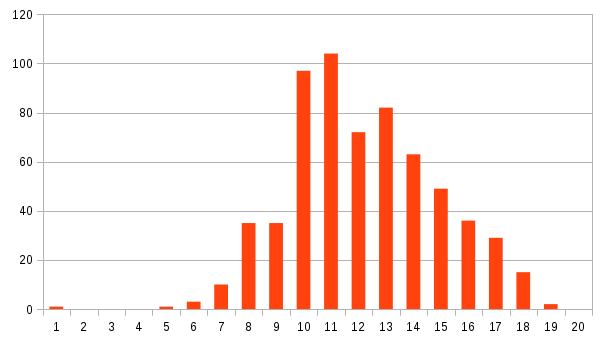
\includegraphics[scale=0.6]{por-chart.png}
\centering
\caption{Grade Distribution for Portuguese}
\end{figure}
\subsubsection{Parameter Values}
\begin{table}[h]

\begin{tabular}{| c | c | c | c | p{3cm} | c | c | c |}
\hline \textbf{min\_thresh} & \textbf{hidden} & \textbf{learn\_rate} & \textbf{momentum} & \textbf{removed} & \textbf{iterations} & \textbf{PassAcc} & \textbf{GradeAcc}\\
\hline 0.025 & \{15,10\} & 0.3 & 0.8 & \_G1 \_G2 \_ & 1 & 87\% & 36\%\\
\hline 0.020 & \{15,10\} & 0.3 & 0.8 & \_G1 \_G2 \_ & 6 & 87\% & 36\%\\
\hline 0.015 & \{15,10\} & 0.3 & 0.8 & \_G1 \_G2 \_ & 17 & 86\% & 39\%\\
\hline 0.01 & \{15,10\} & 0.3 & 0.8 & \_G1 \_G2 \_ & 300 & 88\% & 42\%\\
\hline 0.005 & \{15,10\} & 0.3 & 0.8 & \_G1 \_G2 \_ & 650 & 86\% & 37\%\\
\hline 0.0009 & \{15,10\} & 0.3 & 0.8 & \_G1 \_G2 \_ & 2182 & 79\% & 32\%\\
\hline
\end{tabular}
\caption{Error Threshold Analysis}
\end{table}

\paragraph{Results}
Analysing the table above we can conclude that the best error threshold is 0.01 and for thresholds lower than 0.01 over-fitting effects start to appear.

\subsubsection{Deprecated Inputs}
\begin{table}[H]
\begin{tabular}{| c | c | c | c | p{3cm} | c | c | c |}
\hline \textbf{min\_thresh} & \textbf{hidden} & \textbf{learn\_rate} & \textbf{momentum} & \textbf{removed} & \textbf{iterations} & \textbf{PassAcc} & \textbf{GradeAcc}\\
\hline 0.01 & \{1\} & 0.3 & 0.8 & \_G1 \_G2 \_ & 263 & 86\% & 41\%\\
\hline 0.01 & \{1\} & 0.3 & 0.8 & \_sex \_age \_address \_health \_G1 \_G2 \_ & 374 & 87\% & 42\%\\
\hline 0.01 & \{1\} & 0.3 & 0.8 & \_sex \_age \_address \_activities \_nursery \_romantic \_health \_G1 \_G2 \_ & 516 & 87\% & 42\%\\
\hline 0.01 & \{1\} & 0.3 & 0.8 & \_sex \_age \_address \_Pstatus \_Medu \_Fedu \_Mjob \_Fjob \_activities \_nursery \_romantic \_goout \_health \_G1 \_G2 \_ & 1899 & 86\% & 34\%\\
\hline 0.01 & \{1\} & 0.3 & 0.8 & \_sex \_age \_address \_guardian \_studytime \_failures \_schoolsup \_famsup \_activities \_nursery \_romantic \_goout \_health \_G1 \_G2 \_ & 1269 & 85\% & 35\%\\
\hline 0.01 & \{1\} & 0.3 & 0.8 & \_sex \_age \_address \_paid \_activities \_nursery \_higher \_romantic \_goout \_Dalc \_health \_absences \_G1 \_G2 \_ & 860 & 85\% & 35\%\\
\hline
\end{tabular}
\caption{Deprecated Inputs Analysis}
\end{table}

\begin{table}[H]
\begin{tabular}{| c | c | c | c | p{3cm} | c | c | c |}
\hline \textbf{min\_thresh} & \textbf{hidden} & \textbf{learn\_rate} & \textbf{momentum} & \textbf{removed} & \textbf{iterations} & \textbf{PassAcc} & \textbf{GradeAcc}\\
\hline 0.01 & \{1\} & 0.3 & 0.8 & \_sex \_age \_address \_Pstatus \_Medu \_Fedu \_Mjob \_Fjob \_guardian \_studytime \_failures \_schoolsup \_famsup \_paid \_activities \_nursery \_higher \_romantic \_goout \_Dalc \_health \_absences \_G1 \_G2 \_ & 20000 & 85\% & 36\%\\
\hline 0.01 & \{1\} & 0.3 & 0.8 & \_school \_sex \_age \_address \_famsize \_reason \_traveltime \_activities \_nursery \_internet \_romantic \_famrel \_freetime \_goout \_Walc \_health \_G1 \_G2 \_ & 5218 & 83\% & 38\%\\
\hline 0.01 & \{1\} & 0.3 & 0.8 & \_sex \_age \_address \_famsize \_reason \_activities \_nursery \_romantic \_freetime \_goout \_Walc \_health \_G1 \_G2 \_ & 901 & 86\% & 40\%\\
\hline 0.01 & \{1\} & 0.3 & 0.8 & \_sex \_age \_address \_reason \_paid \_activities \_nursery \_romantic \_freetime \_goout \_Walc \_health \_G1 \_G2 \_ & 648 & 86\% & 43\%\\
\hline
\end{tabular}
\caption{Deprecated Inputs Analysis (Cont.)}
\end{table}


\paragraph{Results}
Following our analysis for the Maths data set we expect that the inputs \textit{sex}, \textit{age}, \textit{address}, \textit{health} to not influence the neural net accuracy. As we can see our hypotheses is correct as the accuracy results without those inputs is maintained.
We also expect that the inputs \textit{romantic}, \textit{nursery} and \textit{activities} won't have an impact on the neural net accuracy, and looking at the experiment accuracy values we can see that it does not affect the accuracy.

Some of the inputs we intuitively mark as important are \textit{Pstatus}, \textit{Medu}, \textit{Fedu}, \textit{Mjob}, \textit{Fjob}, \textit{guardian}, \textit{studytime}, \textit{failures}, \textit{schoolsup}, \textit{famsup},\textit{paid}, \textit{absences}, \textit{Dalc} and \textit{higher}.
We made some experiments to see if the inputs we identified as important are actually of importance to the neural net accuracy. By removing some of them from the neural net inputs, we see a clear decrease in \textit{GradeAcc} leading us to conclude that these inputs are in fact important.

To identify any other important inputs we create a network with only the inputs we intuitively identified as important and compare the network accuracy with the accuracy we have been getting until now. When running an experiment with only the inputs we considered important the net accuracy decreased leading us to believe some important inputs were left out, some more experiments were made to identify them.

Adding the inputs \textit{school}, \textit{traveltime}, \textit{internet} and \textit{famrel} we saw an increase in 2\% comparing this result with the previous experiment.
We kept doing some experiments by removing certain inputs and got a good increase when removing the input \textit{paid}, we can then conclude that having extra paid classes for the Portuguese subject is not strictly related with the final grade and introduces confusion on the network.

\subsubsection{Neural Net Structure}
\begin{table}[H]
\begin{tabular}{| c | c | c | c | p{3cm} | c | c | c |}
\hline \textbf{min\_thresh} & \textbf{hidden} & \textbf{learn\_rate} & \textbf{momentum} & \textbf{removed} & \textbf{iterations} & \textbf{PassAcc} & \textbf{GradeAcc}\\
\hline 0.01 & \{1\} & 0.3 & 0.8 & \_sex \_age \_address \_reason \_paid \_activities \_nursery \_romantic \_freetime \_goout \_Walc \_health \_G1 \_G2 \_ & 648 & 86\% & 43\%\\
\hline 0.01 & \{15\} & 0.3 & 0.8 & \_sex \_age \_address \_reason \_paid \_activities \_nursery \_romantic \_freetime \_goout \_Walc \_health \_G1 \_G2 \_ & 580 & 86\% & 43\%\\
\hline 0.01 & \{15,10\} & 0.3 & 0.8 & \_sex \_age \_address \_reason \_paid \_activities \_nursery \_romantic \_freetime \_goout \_Walc \_health \_G1 \_G2 \_ & 528 & 86\% & 42\%\\
\hline 0.01 & \{20,15,10\} & 0.3 & 0.8 & \_sex \_age \_address \_reason \_paid \_activities \_nursery \_romantic \_freetime \_goout \_Walc \_health \_G1 \_G2 \_ & 555 & 85\% & 42\%\\
\hline 0.01 & \{15,10,5\} & 0.3 & 0.8 & \_sex \_age \_address \_reason \_paid \_activities \_nursery \_romantic \_freetime \_goout \_Walc \_health \_G1 \_G2 \_ & 563 & 86\% & 43\%\\
\hline
\end{tabular}
\caption{Net Structure Analysis}
\end{table}
\paragraph{Results}
After experiments with different net structures we can observe that both the \textit{PassAcc} and \textit{GradeAcc} have no major change, leading us to believe that only one hidden layer with 1 node is sufficient for the network to be as accurate as it can be with the data set provided.


\subsubsection{Momentum and Learning Rate}
\begin{table}[H]
\begin{tabular}{| c | c | c | c | p{3cm} | c | c | c |}
\hline \textbf{min\_thresh} & \textbf{hidden} & \textbf{learn\_rate} & \textbf{momentum} & \textbf{removed} & \textbf{iterations} & \textbf{PassAcc} & \textbf{GradeAcc}\\
\hline 0.01 & \{1\} & 0.3 & 0.1 & \_sex \_age \_address \_reason \_paid \_activities \_nursery \_romantic \_freetime \_goout \_Walc \_health \_G1 \_G2 \_ & 592 & 86\% & 42\%\\
\hline 0.01 & \{1\} & 0.3 & 0.5 & \_sex \_age \_address \_reason \_paid \_activities \_nursery \_romantic \_freetime \_goout \_Walc \_health \_G1 \_G2 \_ & 680 & 87\% & 42\%\\
\hline 0.01 & \{1\} & 0.3 & 0.9 & \_sex \_age \_address \_reason \_paid \_activities \_nursery \_romantic \_freetime \_goout \_Walc \_health \_G1 \_G2 \_ & 659 & 87\% & 41\%\\
\hline 0.01 & \{1\} & 0.1 & 0.1 & \_sex \_age \_address \_reason \_paid \_activities \_nursery \_romantic \_freetime \_goout \_Walc \_health \_G1 \_G2 \_ & 1510 & 86\% & 43\%\\
\hline 0.01 & \{1\} & 0.5 & 0.1 & \_sex \_age \_address \_reason \_paid \_activities \_nursery \_romantic \_freetime \_goout \_Walc \_health \_G1 \_G2 \_ & 425 & 87\% & 42\%\\
\hline 0.01 & \{1\} & 0.9 & 0.1 & \_sex \_age \_address \_reason \_paid \_activities \_nursery \_romantic \_freetime \_goout \_Walc \_health \_G1 \_G2 \_ & 262 & 85\% & 41\%\\
\hline
\end{tabular}
\caption{Momentum and Learning Rate Analysis}
\end{table}
\paragraph{Results}
From the experiences above we can see that the momentum mainly changes the number of iterations, a high momentum can lead the algorithm to overshoot the solution many times but a very low momentum prevents the algorithm to reach the solution faster. As for the leaning rate the same conclusions can be made but in a greater scale, a low learning rate of 0.1 needs 1510 iterations to converge to a solution and as we increase the learning rate the number of iterations decrease.

The values chosen for the learning rate and momentum must be an equilibrium, they must not be so low that converging takes a huge number of iterations nor so high that the solution is overshoot many times before converging.
\newpage
\section{Final Conclusions}

So far we have learned how a neural network is structured, how the back-propagation algorithm works and how to differently train networks in order to achieve different results.

We learned that when solving a problem with neural networks, the data-set must be large enough, for meaningful results. Also, when building a data-set from a questionnaire, one must always keep in mind that the participants may have lied.

Learning this subject was fun because of how easy it is to be impressed by machine learning through training. And now we have some knowledge of how it works.
\section{Improvements}

\section{Resources}

\subsection{Bibliography}

\url{https://web.fe.up.pt/~eol/IA/1516/APONTAMENTOS/7_RN.pdf}

\href{https://www.youtube.com/watch?v=q0pm3BrIUFo}{Neural Nets, Back Propagation, Patrick Winston, M.I.T.}

\url{http://www.faqs.org/faqs/ai-faq/neural-nets/}

\url{http://stats.stackexchange.com/questions/181/how-to-choose-the-number-of-hidden-layers-and-nodes-in-a-feedforward-neural-netw}

\url{http://www.akamaiuniversity.us/PJST9_1_72}

\url{https://takinginitiative.wordpress.com/2008/04/23/basic-neural-network-tutorial-c-implementation-and-source-code/}

\url{https://github.com/harthur/brain}

\subsection{Software}

To train the network, we will use the javascript framework \href{https://github.com/harthur/brain}{\textbf{BrainJS}}, an open source implementation of a neural network, using the back-propagation algorithm, implemented using the basic sigmoid function.

\newpage
\section{Appendix}
In this section we present the different interface menus.

\begin{figure}[H]
\label{fig:example}

\includegraphics[scale=0.3]{interface0.png}
\centering
\caption{User can either create network from data set or load existing network.}
\end{figure}

\begin{figure}[H]
\label{fig:example}
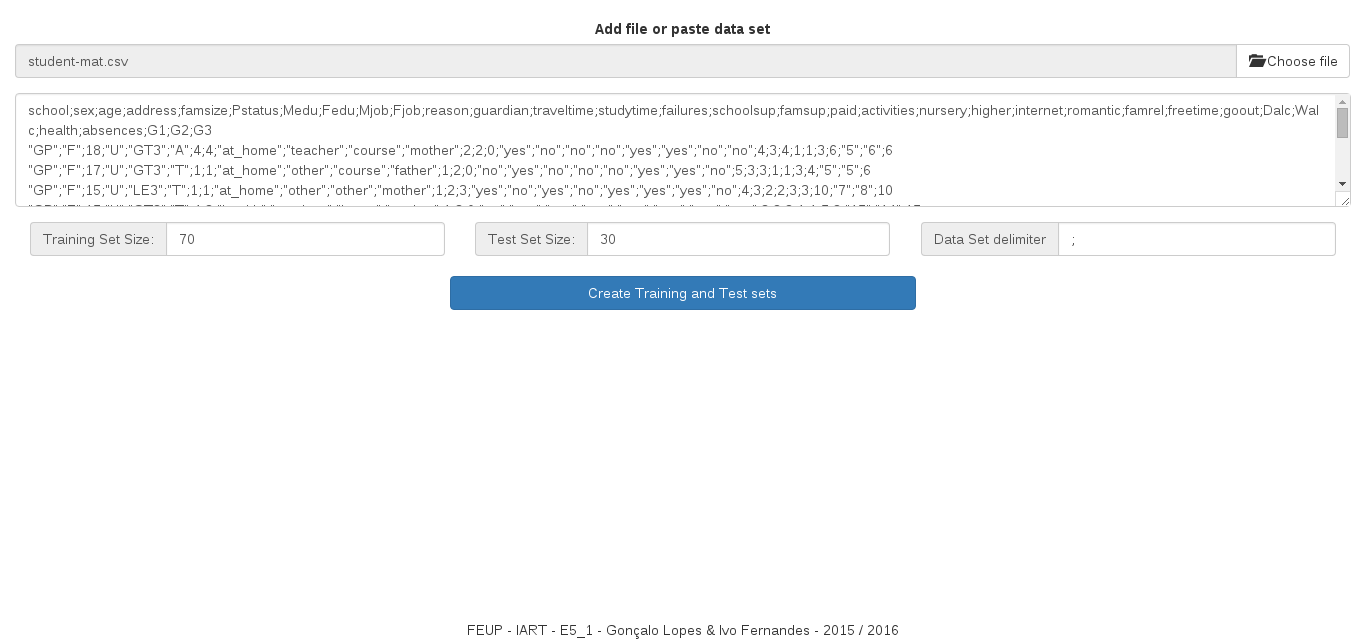
\includegraphics[scale=0.3]{interface1.png}
\centering
\caption{Create network interface.}
\end{figure}

\begin{figure}[H]
\label{fig:example}
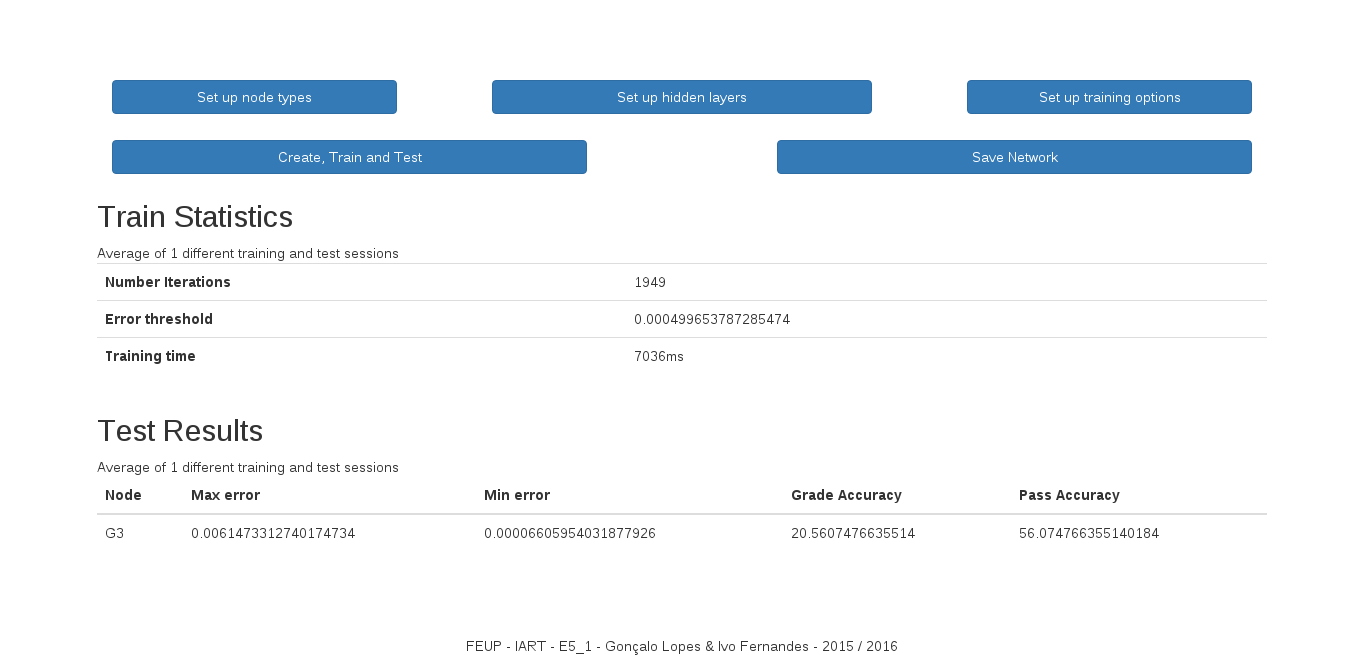
\includegraphics[scale=0.3]{interface2.png}
\centering
\caption{Train and test results and training options.}
\end{figure}

\begin{figure}[H]
\label{fig:example}
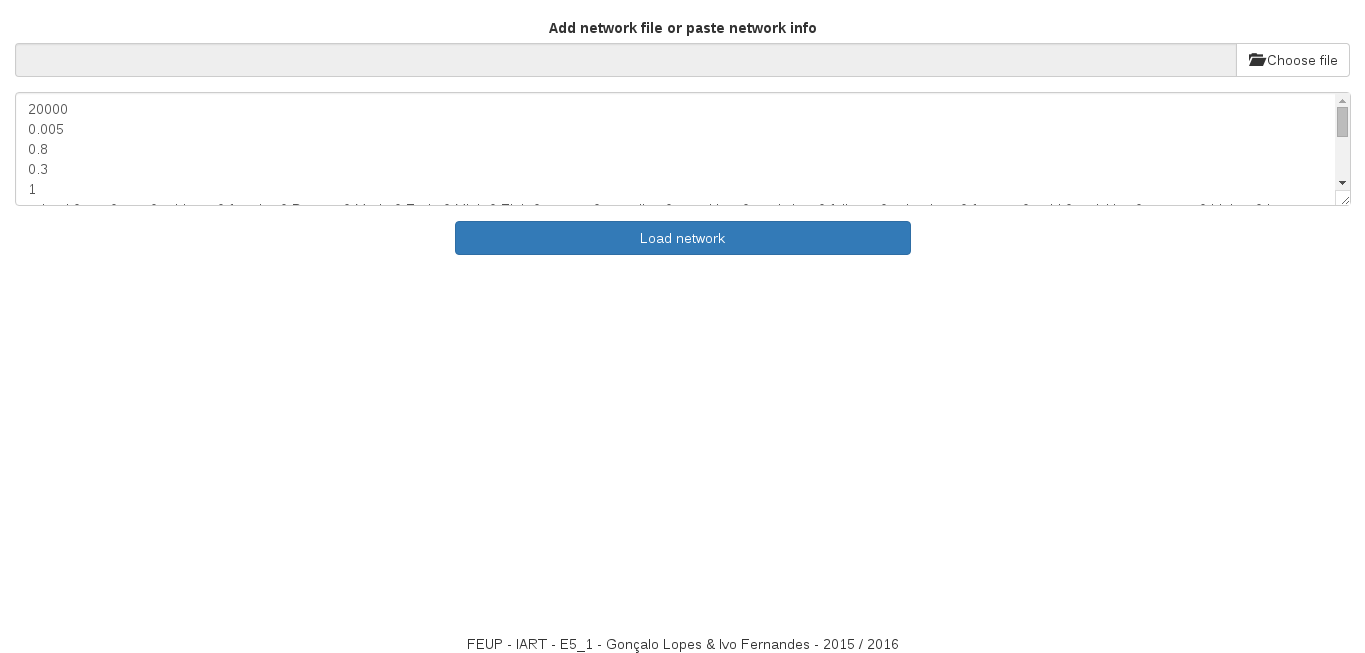
\includegraphics[scale=0.3]{interface3.png}
\centering
\caption{Load network interface.}
\end{figure}
\end{document}
